\chapter{Lecture 13 - Recompressing, Regenerating S-CO$_{2}$ Cycle}
\label{ch:ch13}
\section{Objectives}
The objectives of this lecture are:
\begin{enumerate}
\item Give a detailed description of the analysis method for the RRS-CO$_{2}$ Brayton cycle
\item Discuss the MATLAB implementation of the solution
\end{enumerate}

\index{Brayton cycle, recompressing regenerating S-CO$_{2}$}
\section{Recompressing Regenerating S-CO$_{2}$ Brayton Cycle}
\newthought{A schematic of this cycle} is given in Figure \ref{fig:rrsco2_schematic}. In order to better match the temperature change on the cold- and hot- side of the regenerators, a portion of the working fluid bypasses the pre-cooler, compressor and low-temperature regenerator; instead it is recompressed and mixed with fluid leaving the low-temperature regenerator at state point 3.  The combined flow is pre-heated in the high-temperature regenerator before heat addition from the reactor.


\begin{figure}
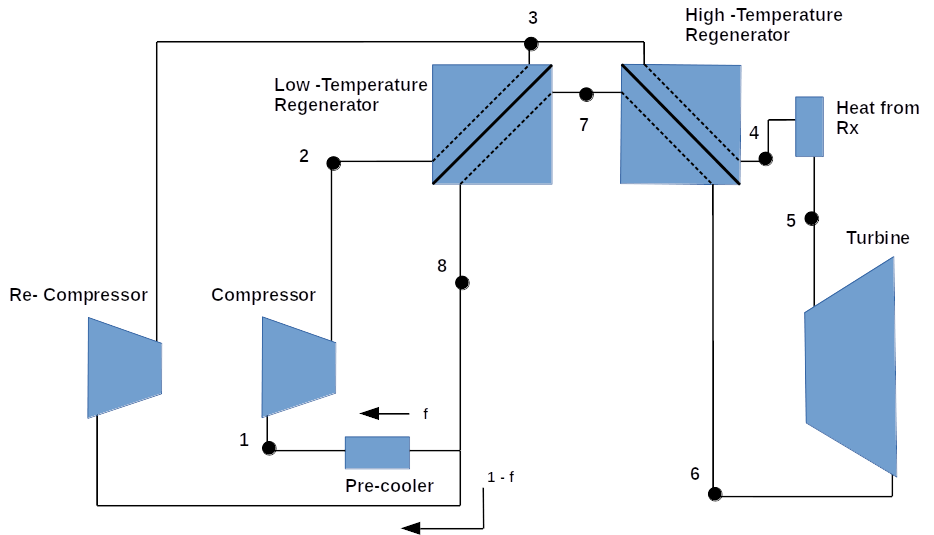
\includegraphics{rrsco2_schematic.png}
\caption{Schematic RR S-CO$_{2}$ Brayton cycle.}
\label{fig:rrsco2_schematic}
\end{figure}

\newthought{Compared to } some of the more complex Rankine cycles analyzed in earlier lectures, this cycle is relatively simple with only 8 state points.  Still, there are some challenges to be overcome.  Let us suppose that we know the minimum and maximum pressure and temperature for the working fluid; we know the isentropic efficiency of the turbine and both compressors; and we can assume a value of regenerator effectiveness for both the low- and high-temperature regenerators.
\begin{itemize}
\item with the aforementioned given data, we should be able to calculate thermodynamic properties at state point 1 and 2 along with 5 and 6. 
\item If we do not know the flow fraction $f$ of working fluid going through the pre-cooler---and why would we?---then we cannot calculate the temperature or enthalpy of state point 3;
\item without knowing the temperature or enthalpy of state point 3, we cannot calculate properties of state point 4, 7, or 8 either.
\end{itemize}
We have a total of 5 unknown properties---f, and the enthalpy/temperature of state points 3,4,7, and 8---and thus need to develop 5 independent relationships.  As with previous cycles, these equations in general will be non-linear and values of the dependent variables need to be constrained to ensure a physically meaningful solution.  We will form these equations using the following relationships:\marginnote[1.5cm]{\textbf{Note: }The equations are all re-arranged in the MATLAB code to facilitate use with FMINCON.  

Partial MATLAB code listing provided for clarity/completeness. A full MATLAB script to carry out this analysis is provided in the appendices.}
\begin{enumerate}
\item Low-temperature regenerator effectiveness:
$$\eta_{\text{LTR}} = \frac{h_7 - h_8}{h_7-h_{(P_8,T_2)}}$$
\begin{lstlisting}
%f = [flow fraction, h(3), h(4), h(7), h(8)]
gas = py.EasProp.simpleFluid('CO2','SI');
LTR_eff_eq = @(f) eta_LTR*(f(4) - ...
    gas.h_pT(P(8),T(2)))-(f(4)-f(5));
\end{lstlisting}

\item High-temperature regenerator effectiveness:
$$\eta_{\text{HTR}} = \frac{h_6 - h_7}{h_6 - h_{(P_7,T_2)}}$$
\begin{lstlisting}
%f = [flow fraction, h(3), h(4), h(7), h(8)]
HTR_eff_eq = @(f) eta_HTR*(h(6) - ...
    gas.h_pt(P(7),gas.T_ph(P(3),f(2))))-(h(6)-f(4));
\end{lstlisting}

\item Low-temperature regenerator energy balance:
$$f(h_3 - h_2) = h_7 - h_8$$
\begin{lstlisting}
%f = [flow fraction, h(3), h(4), h(7), h(8)]
LTR_ebal = @(f) f(1)*(f(2)-h(2))-(f(4)-f(5));
\end{lstlisting}

\item High-temperature regenerator energy balance:
$$h_4 - h_3 = h_6 - h_7$$

\begin{lstlisting}
%f = [flow fraction, h(3), h(4), h(7), h(8)]
HTR_ebal = @(f) (f(3)-f(2) - (h(6)-f(4));
\end{lstlisting}
\item The last relationship will be that the state of the fluid at exit from the low-temperature regenerator is the same as the state of the fluid discharged from the re-compressor.  On the schematic, both of these flows correspond to state point 3:
$$h_3 = h_8 - \frac{h_8 - h_{3s}}{\eta_{RC}}$$
where the left hand side is derived from a standard analysis of compressor work for the re-compressor.  Note for this equation, we do not know $h_{3s}$ and we do not want to add it to our list of unknown variables.  Instead we will re-express $h_{3s}$ in terms of what we do know along with existing unknowns:
$$h_{3s} = h_8 - \frac{h_8 - (h_8 - \overbrace{h(P_3,\overbrace{s(P_8,h_8)}^{s_8})}^{h_{3s}})}{\eta_{RC}}$$

\begin{lstlisting}
%f = [flow fraction, h(3), h(4), h(7), h(8)]
sp3_ident = @(f) f(5) - ...
    (f(5) - gas.h_ps(P(3),gas.s_ph(P(8),f(5))))/eta_rc - f(2);
\end{lstlisting}


\end{enumerate}
The five equations are then combined into a single balance equation for use with FMINCON.

\begin{lstlisting}
balance = @(f) abs(LTR_eff_eq(f)) + abs(HTR_eff_eq(f)) + ...
    abs(LTR_ebal(f)) + abs(HTR_ebal(f)) + abs(sp3_ident(f));
\end{lstlisting}

\newthought{We also need} to provide constraints to help ensure that FMINCON arrives at a physically meaningful solution. A table of possible constraints and starting values are provided in Table \ref{tb:rrsco_constraints}. These are encoded in MATLAB as follows:
\begin{margintable}
\begin{tabular}{lc}
\toprule
Constraint & Starting Value \\
\midrule
$0 \le f \le 1$ & 0.5 \\
$h_2 \le h_3 \le h_6$ & $h_2$ \\
$h_2 \le h_4 \le h_5$ & $h_5$ \\
$h_1 \le h_7 \le h_6$ & $h_6-1$ \\
$h_2 \le h_8 \le h_6$ & $h_2$ \\
\bottomrule
\end{tabular}
\caption{Constraints and starting values for cycle analysis.}
\label{tb:rrsco_constraints}
\end{margintable}

\begin{lstlisting}
%f = [flow fraction, h(3), h(4), h(7), h(8)]
lbound = [0 h(2) h(2) h(1) h(2)];
ubound = [1 h(6) h(5) h(6) h(6)];
Xo = [0.5 h(2) h(5) h(6)-1 h(2)];
\end{lstlisting}

\subsection{Results}
\newthought{As a reminder,} our goal was to reduce exergy destruction in the regenerator for a supercritical CO$_{2}$ Brayton cycle and thereby increase cycle thermal efficiency.  Results of the analysis are shown in Figure \ref{fig:rrsco2_results}. 
\begin{marginfigure}
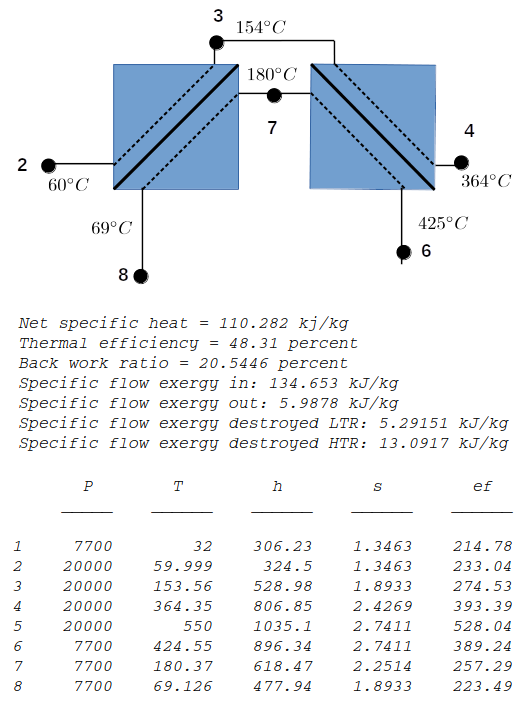
\includegraphics{rrsco2_results.png}
\caption{Calculated results for RR S-CO$_{2}$ cycle.}
\label{fig:rrsco2_results}
\end{marginfigure}
We can see that the thermal efficiency is increased to 48.3\% and that the temperature differences at each side of the regenerators is reduced.  The largest differential temperature is at the high-temperature regenerator with state points 4 and 6 roughly 60 degrees different. It corresponds, therefore that the higher rate of exergy destruction is in the high-temperature regenerator.  The net specific work (and heat) is reduced because the specific work of the re-compressor is elevated since it is compressing working fluid that has not been pre-cooled.  


